%%%%%%%%%%%%%%%%%%%%%%%%%
% Dokumentinformationen %
%%%%%%%%%%%%%%%%%%%%%%%%%
\newcommand{\titleinfo}{Elekrische Maschinen - Formelsammlung}
\newcommand{\authorinfo}{F. Braun, L. Schmid, U. Giger, R. Koller, S.
Arnold, S. Ferreti}
\newcommand{\versioninfo}{$Revision: 975 $ - powered by \LaTeX}

%%%%%%%%%%%%%%%%%%%%%%%%%%%%%%%%%%%%%%%%%%%%%
% Standard projektübergreifender Header für
% - Makros 
% - Farben
% - Mathematische Operatoren 
%
% DORT NUR ERGÄNZEN, NICHTS LÖSCHEN
%%%%%%%%%%%%%%%%%%%%%%%%%%%%%%%%%%%%%%%%%%%%%  
\include{header/header}


% Setzt ein zentriertes Bild mit Beschriftung --> DANKE UELI!!!
% Syntax: \abb{Pfad zum Bild}{Bildgrösse}{Beschriftung des Bildes}
\newcounter{abbildungen} \stepcounter{abbildungen}
\newcommand{\abb}[3]{
\begin{center}
\includegraphics[width=#2]{#1} \\
Abbildung \arabic{abbildungen}: #3 
\stepcounter{abbildungen}    
    \end{center}
}

% Möglichst keine Ergänzungen hier, sondern in header.tex
\begin{document}


%%%%%%%%%%%%%%%%%%%%%%%%%%%%%%%%%%%%%%%%%%%%%%%%%%%%%%%%%%%%%%%%%%%%%%%%%%%%%%%%%%%%%%%%%%%%%%%
%%%%%%%%%%%%%%%%%%%%%%%%%%%%%%%%%%%%%%%%%%%%%%%%%%%%%%%%%%%%%%%%%%%%%%%%%%%%%%%%%%%%%%%%%%%%%%%
\section{Generelle Eigenschaften el. Maschinen}
\subsection{Generelle Formeln von el. Maschinen}
\renewcommand{\arraystretch}{2}
	\begin{tabular}[c]{ | p{5cm} | p{8cm} | p{4cm} | }
		\hline
		\textbf{Name} & \textbf{Formel} & \textbf{Einheit}\\    
		\hline
		Permeabilität
		& $\mu = \mu_0 \mu_r = \mu_r \cdot 4 \cdot \pi \cdot 10^{-7}
		\frac{Vs}{Am} = \mu_r \cdot 1.2566 \frac{\mu H}{m}=\frac{B}{H}$ &$\frac{\mu
		H}{m}=\frac{Vs}{An}$\\
		\hline 
		Magn. Flussdichte %B = \frac{\mu}{4 \pi} \cdot \frac{Q v}{r^2} =
		& $B = \frac{F}{Q \cdot v} = H \cdot \mu \text{\qquad wobei } \vec{v} \perp
		\vec{B}$ & $\frac{Vs}{m^2} = T$ (Tesla) \\
		\hline
		Lorentzkraft
		& $\vec{F} = Q (\vec{v} \times \vec{B})=I(\vec{l}\times \vec{B}) \hspace{1cm} |\vec{F}| = Q \cdot v \cdot B
		\cdot \sin\alpha$
		&$N$\\
		Ampèresches Gesetz
		&$F=\frac{Q_2 \cdot v_2 \cdot Q_1 \cdot v_1 \cdot \mu}{r^2 \cdot 4\pi}$
		&\\
		\hline
		Drehmoment von Schleifen
		& $M_{max} = 2 \cdot F \cdot \frac{d}{2}= F \cdot d = N \cdot B \cdot
		I \cdot d \cdot l = \frac{P_{Mech}}{2 \pi n_0} $
		& Nm; $n_0= Drehzahl$\\
		\hline
		\textbf{3-Finger-Regel:}
		(rechte Hand)
		& $F$ = Daumen, $v$ = Zeigefinger, $B$ = Mittelfinger
		& Bei $Q < 0$ wechselt Richtung von B!\\
		\hline
		Magnetische Feldstärke
		& $\vec{H} = \frac{ \vec{B}}{\mu }$
		& $\frac{A}{m}$\\
		Magnetische Spannung
		& $V_{mAB} = \int\limits \vec{H}(s) \cdot \vec{ds}$ ($V_m$ ist abhängig vom
		Weg) & $A$ \\
		\hline
		Durchflutung
		& $\Theta = \oint\vec{H} \cdot \vec{ds} = \sum\limits_{x=1}^n H_x \cdot l_x = \int\limits \vec{J}
		\cdot \vec{dA} \vee \underbrace{\sum I_k}_{= N I} = V_m$
		& $A$\\
		\hline
		Magnetischer Fluss
		& $\Phi = \int \vec{B} \vec{dA}$
		& $Vs = Wb$ (Weber)\\
		& $\Phi = B \cdot A \cdot \cos(\gamma)=b \cdot A \cdot (1+Streufluss)$
		& B homogen\\
		\hline
		\textbf{Maxwell-Gesetz}
		& $\oint \vec{B} \vec{dA} = 0$ (vgl. Kirchhoff 1 ($\sum I = 0$))
		&\\
		\hline
		Füllfaktor
		&$F=\frac{A_{Effektiv Fe}}{A_{Tot}}$
		& $[-]$\\
		\hline
		Magn. Widerstand
		& $R_m = \frac{V_m}{\Phi} = \frac{\Theta}{\Phi} = \frac{l}{\mu A} $
		& $\frac{A}{Wb}$ \\
		\hline
		Magn. Leitwert
		& $\Lambda = \frac{1}{R_m} = \frac{\Phi}{V_m}=\frac{\Phi}{\Theta}$
		& $\frac{Vs}{A} = H$ (Henry) (Im Formelbuch als $A_L$)\\
		\hline
		Verketteter Fluss
		& $\Psi = \sum \Phi $ (meist $\Psi = N \Phi$)
		& $[\Psi] = [\Phi] = Vs = Wb$\\
		\hline
		Induktivität
		& $L = \frac{\Psi}{I}  \qquad \text{Bei idealer Koppl.: } L = \Lambda N^2 = \frac{N^2}{R_m} $
		& $[L] = \frac{Vs}{A} = H$\\
		\hline
		Gegeninduktivität
		& $M = M_{21} = M_{12}$ Bei idealer Koppl. $M = \sqrt{L_1 L_2}$
		& vorder Index = Wirkung,\\
		&$M_{21} = \frac{\Psi_{21}}{I_1}$  (meist $M_{21} = \frac{N_2 \Phi_{21}}{I_1}$)
		& hinterer = Ursache\\
		\hline
		Kopplungsfaktor
		& $k = \frac{M}{\sqrt{L_1 L_2}}$ Bei idealer Kopplung: $k = 1$
		& $[-]$ \\
		\hline
		Streukoeffizient
		& $\sigma = 1 - k^2 = 1 -\frac{M^2}{L_1 L_2}$ Bei idealer Kopplung: $\sigma = 0$
		& $[-]$\\
		\hline
		Kreis-r in M-Feld abgelenkte Q
		& $r = \frac{m_Q \cdot v}{Q \cdot B}$
		&m, $ m_e = 9,11 \cdot 10^{-31} kg$ \\
		\hline
		Spannung
		& $U = L \cdot \frac{di}{dt}=N \cdot B \cdot l \cdot v$
		& V\\
		\hline
		Wirkungsgrad
		& $\eta = \frac{P_2}{P_1}=\frac{abgegebene P}{aufgenommene P}= \frac{P_1 -
		P_Verluste}{P_1}$
		& -\\
		\hline
		Verluste:
		&Hysterese 	$\sim f \cdot B^2$ \qquad
		Wirbelstrom $\sim f^2 \cdot B^2$ \qquad
		Lüfter	$	\sim n^3$ \qquad\qquad
		Erreger$		= I_E ^2 \cdot R_e $&\\
		\hline
	\end{tabular}
	\renewcommand{\arraystretch}{1}	
	
	\subsection{Übersicht über Motorenarten}
		\abb{Bilder/uebersicht_el.png}{11cm}{Prinzipieller Aufbau El. Maschinen}

\section{Gleichstrommaschinen (GSM)}
	\subsection{Funktionsprinzip}
		Ein Gleichstrom ist im Prinzip eigendlich nur eine stromdurchflossene
		Schleife, welche sich in einem Magnetfeld befindet.\\
		Durch die Lorenzkraft wirkt auf die Schleife ein Drehmoment, welche sie in
		eine maximal halbe Drehung versetzt.
		Danach muss man den Schleifenstrom umpolisieren, um die Drehung weiter zu
		führen.\\
		\abb{Bilder/GSM_Funktion.png}{14cm}{Funktion eines GSM mit Stromwender}
		\abb{Bilder/GSM_Ersatz.png}{14cm}{Erstzschema der 4 Schaltungsarten}
		A1,A2: Ankerwicklung, B1,B2: Wendepolwicklung, C1,C2: Kompensationswicklung, \\
		D1,D2: Reihenschlusswicklung, E1,E2: Nebenschlusswicklung, F1,F2: Fremderregte Wicklung
		
		Um ein gleichmässiges Drehmoment erreichen zu können, kann folgende Wicklung
		angewendet werden\\
		\begin{minipage}{10cm}
			\abb{Bilder/GSM_Wicklungen}{9.5cm}{Entstehung eienr Schleifenwicklung}
		\end{minipage}
		\begin{minipage}{7cm}
			\abb{Bilder/GSM_Drehmomentdarstellung}{6.5cm}{Alle Drehmomente
			zusammen ergeben ein gleichmässiges Drehmoment}
		\end{minipage}
		
	\subsection{Nebenschluss Maschinen}

		\begin{tabular}[c]{ | p{6cm} | p{9cm} |}
			\hline
			Drehzahl
			& $ n= \frac{U}{k_1 \cdot \Phi} - \frac{R_A \cdot M}{k_1 \cdot k_2 \cdot
			\Phi^2} \sim \frac{U}{I_E} - \frac{M}{I_E^2}$\\ 
			& $\Longrightarrow $ bei $I_E$ = 0 und $M$ = 0 $n \rightarrow \infty$\\
			\hline
			Drehmoment
			& $M=\frac{k_2 \cdot \Phi \cdot U_{Anker}}{R_{Anker}} - \frac{k_1 \cdot k_2
			\cdot\phi^2 \cdot n}{R_A} =\frac{P_{mech}}{2\pi
			n_N}=\frac{U_{iN}I_N}{2\pi n_N}\sim I_E \cdot U_A - I_E ^2 \cdot n$\\
			\hline
			Leistung
			& $P_{Anker}= U_i \cdot I \pm I^2 \cdot R_A $(+ bei Motor; - bei Generator)\\
			\hline
			Anlaufmoment
			& $M_A = \frac{k_1 \cdot \Phi \cdot U}{R_1}$\\
			\hline
			Leerlaufmoment
			& $n_0 = \frac{U}{k_1 \cdot \Phi}$\\
			\hline
		
		\end{tabular}

	\subsection{Reihenschluss Maschine}

		\begin{tabular}[c]{ | p{6cm} | p{9cm} |}
		\hline
		Drehmoment
		& $ M=  \frac{U_{Induziert} \cdot I_A}{2 \cdot \pi n_N} = \frac{k_1 \cdot k_E
		\cdot I_A ^2}{2\cdot \pi n_N}= \frac{k_1 \cdot k_E}{2 \cdot
		\pi n_N}\cdot(\frac{U}{R_A + R_E + k_1 \cdot k_E \cdot n})^2$\\
		\hline
		Anlaufstrom
		& $I_A=\frac{U_N}{\sum R_a}=\frac{U_N I_N^2}{U_N I-P_N}$\\
		\hline
		\end{tabular}


\section{Grundlagen Drehfeldmaschinen}
	\subsection{Dreiphasenwechselstrom (Drehstrom)}
		%\subsection{Entstehung des Drehstrom-Systems}
			\begin{tabular}{p{8.5cm}p{9cm}}
	        	\begin{minipage}{8cm}
	            	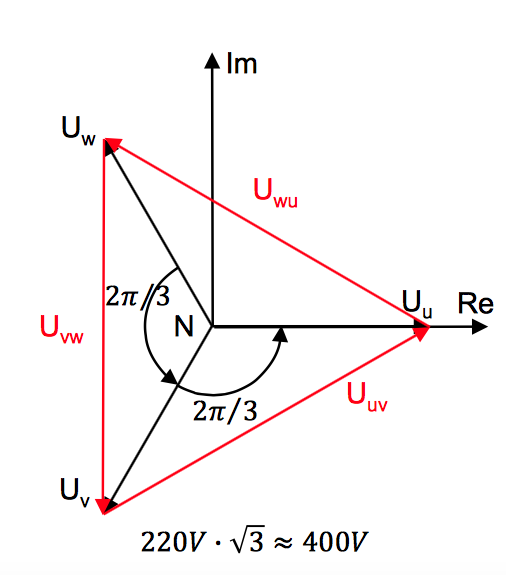
\includegraphics[width=7.5cm]{../WS_DST/bilder/Drehstrom.png}
	            \end{minipage} &
				\begin{minipage}{10cm}
	            	Zeiger drehen mit $\omega t$ im Gegenuhrzeigersinn ($\omega > 0$). \\
	            	$\underline{U}_2$ ist gegenüber $\underline{U}_1$
					$120^{\circ}$ nacheilend, $\underline{U}_3$ gegenüber $\underline{U}_1$ $240^{\circ}$.  \\ \\
					Somit gilt (bei symmetrischer Belastung): \\
					$\underline{U}_2 = \underline{U}_1 \cdot e^{j (-120^{\circ})}; \underline{U}_3
					= \underline{U}_1 \cdot e^{j (-240^{\circ})} = \underline{U}_1 \cdot e^{j
					(120^{\circ})}$
	            \end{minipage}
	        \end{tabular}
	
	% 		\subsubsection{Verketten der Spannungen oder Ströme}
	% 			\begin{tabular}{p{5cm}p{6cm}p{7cm}}
	%             	\textbf{Maschensatz} &
	%             		\fbox{$\underline{U}_1 + \underline{U}_2 + \underline{U}_3 = 0$} \\
	%             	\textbf{Knotenpunktsatz} &
	%             		\fbox{$\underline{I}_1 + \underline{I}_2 + \underline{I}_3 = 0$} \\
	%             \end{tabular}
	
			\subsubsection{Stern- (Y) / Dreieckschaltung ($\Delta$)}
	            	\renewcommand{\arraystretch}{1.5}
				\begin{tabular}{| p{4.5cm} | l | l |}
					\hline
		 				& Sternschaltung (Y)		& Dreieckschaltung ($\Delta$)\\
		 			\hline
		 			\vspace{0.2cm}
		 				%\textbf{Zeigerdiagramm} & & \\
		 				&
		 					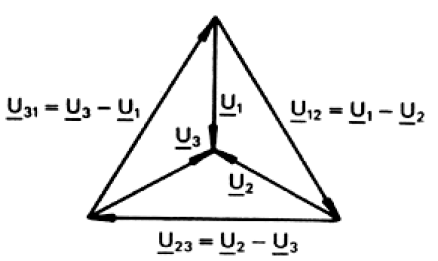
\includegraphics[width=5cm]{../WS_DST/bilder/Sternspannung.png} &
		 					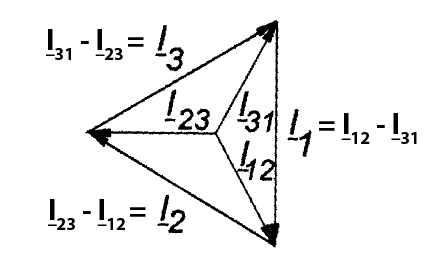
\includegraphics[width=5cm]{../WS_DST/bilder/Dreieckstrom.png} \\
	
			 			Verkettete Spannung &
			 				$U = U_{Str} \cdot \sqrt{3}$ \hspace{0.2cm} $\underline{U} = \underline{U}_{Str} \cdot \sqrt{3} \cdot e^{j 30^\circ}$ &
			 				$U = U_{Str}$ \hspace{0.2cm} $\underline{U} = \underline{U}_{Str}$ \\
			 			Aussenleiterströme &
			 				$I = I_{Str}$ \hspace{0.2cm} $\underline{I} = \underline{I}_{Str}$ &
			 				$I = I_{Str} \cdot \sqrt{3} $ \hspace{0.2cm} $\underline{I} =
			 				\underline{I}_{Str} \cdot \sqrt{3} \cdot e^{-j 30^\circ} $ \\ Gesamt-Scheinleistung &
			 				$S = 3 \cdot S_{Str} =\sqrt{3} \cdot U \cdot I $ \hspace{0.2cm} in $[VA]$
			 				& $S = 3 \cdot S_{Str} = \sqrt{3} \cdot U \cdot I$ \hspace{0.2cm} in $[VA]$ \\ Scheinleistung pro Strang &
			 				\multicolumn{2}{l|}{\hspace{3cm} $S_{Str} = U_{Str} \cdot I_{Str}$ \hspace{0.2cm} in $[VA]$} \\
			 			Wirkleistung &
			 				\multicolumn{2}{l|}{\hspace{3cm} $P = S \cdot \cos\varphi = \sqrt{3} \cdot U \cdot I \cdot \cos\varphi$ \hspace{0.2cm} in $[W]$} \\
			 			Blindleistung &
			 				\multicolumn{2}{l|}{\hspace{3cm} $Q = S \cdot \sin\varphi = \sqrt{3} \cdot U \cdot I \cdot \sin\varphi$ \hspace{0.2cm} in $[var]$} \\
	% 		 			Wirkarbeit &
	% 		 				\multicolumn{2}{l|}{\hspace{3cm} $W = P \cdot t = \sqrt{3} \cdot U \cdot I \cdot cos\varphi \cdot t$ \hspace{0.2cm} in $[Ws, kWh]$} \\
	% 		 				&\multicolumn{2}{c|}{}\\
	% 		 			Blindarbeit &
	% 		 				\multicolumn{2}{l|}{\hspace{3cm} $W_b = Q \cdot t = \sqrt{3} \cdot U \cdot I \cdot sin\varphi \cdot t$ \hspace{0.2cm} in $[varh, kvarh]$} \\
		 			\hline
				\end{tabular}
	        \renewcommand{\arraystretch}{1}
	
% 	        \subsubsection{Ausfall des Neutralleiters: Bestimmung des Y-Punktes mittels Leitwert-Operatoren}
% 	            \begin{tabular}{p{5cm}p{13cm}}
% 	            	\begin{minipage}{8cm}
% 	                	\includegraphics[width=5cm]{../WS_DST/bilder/ZeigerdarstellungVerschobenerSternpunkt.png}
% 	                \end{minipage} &
% 					\begin{minipage}{13cm}
% 	                	$\underline{U}_{12} = \underline{U}_{1N'} - \underline{U}_{2N'}$ \hspace{0.3cm}
% 	                	$\underline{U}_{1N'} = \underline{U}_{1N} + \underline{U}_{NN'}$ \hspace{0.3cm}
% 	                	$\underline{I}_1 = \underline{Y}_1 \cdot \underline{U}_{1N'} = \underline{Y}_1 \cdot (\underline{U}_{1N} + \underline{U}_{NN'})$ \\
% 	                	$\underline{U}_{23} = \underline{U}_{2N'} - \underline{U}_{3N'}$ \hspace{0.3cm}
% 	                	$\underline{U}_{2N'} = \underline{U}_{2N} + \underline{U}_{NN'}$ \hspace{0.3cm}
% 	                	$\underline{I}_2 = \underline{Y}_2 \cdot \underline{U}_{2N'} = \underline{Y}_2
% 	                	\cdot (\underline{U}_{2N} + \underline{U}_{NN'})$ \\ $\underline{U}_{31} = \underline{U}_{3N'} - \underline{U}_{1N'}$ \hspace{0.3cm}
% 	                	$\underline{U}_{3N'} = \underline{U}_{3N} + \underline{U}_{NN'}$ \hspace{0.3cm}
% 	                	$\underline{I}_3 = \underline{Y}_3 \cdot \underline{U}_{3N'} = \underline{Y}_3
% 	                	\cdot (\underline{U}_{3N} + \underline{U}_{NN'})$ \\ \\
% 	                	$$\underline{U}_{NN'} = \boldsymbol{-} \frac{(\underline{Y}_1 \cdot
% 	                	\underline{U}_{1N} + \underline{Y}_2 \cdot \underline{U}_{2N} + \underline{Y}_3 \cdot
% 	                	\underline{U}_{3N})}{\underline{Y}_1 + \underline{Y}_2 +
% 	                	\underline{Y}_3}$$
% 	                \end{minipage}
% 				\end{tabular}
% 	
% 		\subsubsection{Defektleistung von symmetrischen Drehstromverbrauchern}
% 			\begin{tabular}{| p{7.5cm} | l | l |}
% 				\hline
% 	 				& Normalleistung		& Defektleistung\\
% 	 			\hline
% 		 			\textbf{Y-Schaltung bei Leiter- oder Strangausfall} ohne Neutralleiter &
% 		 				$P_{Norm} = 3 \cdot \frac{U^2_{Str}}{R} = \frac{U^2}{R}$ &
% 		 				$P_{Def} = \frac{1}{2} \frac{U^2}{R}$ \tiny{nur 50\% von $P_{Norm}$} \\
% 		 			&&\\
% 		 			\textbf{Y-Schaltung bei Leiter- oder Strangausfall} mit Neutralleiter &
% 		 				$P_{Norm} = 3 \cdot \frac{U^2_{Str}}{R} = \frac{U^2}{R}$ &
% 		 				$P_{Def} = 2 \cdot \frac{U^2_{Str}}{R} = \frac{2}{3} \frac{U^2}{R}$ \tiny{nur 66\% von
% 		 				$P_{Norm}$} \\ &&\\
% 		 			\textbf{$\Delta$-Schaltung bei Leiterausfall} &
% 		 				$P_{Norm} = 3 \cdot \frac{U^2}{R}$ &
% 		 				$P_{Def} = \frac{U^2}{R} + \frac{U^2}{2R} = \frac{3U^2}{2R}$ \tiny{nur 50\% von $P_{Norm}$} \\
% 		 			&&\\
% 		 			\textbf{$\Delta$-Schaltung bei Strangausfall} &
% 		 				$P_{Norm} = 3 \cdot \frac{U^2}{R}$ &
% 		 				$P_{Def} = 2 \cdot \frac{U^2}{R}$ \tiny{nur 66\% von $P_{Norm}$} \\
% 		 		\hline
% 			 \end{tabular}
	
		\subsubsection{Stern-Dreieck-Umwandlung}% \formelbuch{18}}
		%\begin{figure}
		  \begin{minipage}[lt]{7.5 cm}
		    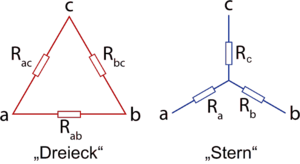
\includegraphics[width=6cm]{../WS_DST/bilder/stern-dreieck.png}
		  \end{minipage}
		  \begin{minipage}[rt]{9.35 cm} %BASTEL!!
	      \renewcommand{\arraystretch}{2}
		  \begin{tabular}{ll}
			Umwandlung $\triangle \rightarrow Y$:
				&$Z_{c} = \dfrac{Z_{ac} Z_{bc}}{Z_{ab}+Z_{bc}+Z_{ac}}$\\
			Umwandlung $Y \rightarrow \triangle$:
				&$Y_{ac}=\dfrac{Y_{a} Y_{c}}{Y_{a}+Y_{b}+Y_{c}}$\\
			Bei gleichen Widerständen:
			&$R_Y = \frac{R_\triangle}{3}$ \\
			Bei gleichen Kapazitäten:
			&$C_Y = C_\triangle \cdot 3 $ \\
			Bei gleichen Induktivitäten:
			&$L_Y = \frac{L_\triangle}{3}$
			  \end{tabular}
		      \renewcommand{\arraystretch}{1}
			  \end{minipage}
			%\end{figure}
	
	\subsection{Feld in einer Drehstrommaschine}
		\begin{minipage}{7cm}
   			\abb{Bilder/Drehfeld.png}{6cm}{Entstehung eines Drehfeldes in einem
   			elMaschine}
        \end{minipage}
		\begin{minipage}{11cm}
	 		Bei einem Drehfeld entsteht zu jedem Zeitpunkt gleichgrosses Magnetisches Feld,
			woraus dann ein gleichmässiges Drehmoment resultieren kann. Nach dem
			obrigen Bild dreht sich das Feld in einer Periode um die eigene Achse. Verwendet
			man mehrere Polpaare wird die Drehzahl reduziert\\
			$Drehfelddrehzahl  = n_d =\frac{f}{p}$ \\
        \end{minipage}
		\subsubsection{Schlupf}
			Als Schlupf bezeichnet man die Beziehung zwischen Drehfelddrehzahl und
			Läuferdrehzahl. Sie wird mit folgender Formel beschrieben:\\
			\begin{minipage}{8cm}
				$Schlupf = s = \frac{n_d - n}{n_d}$\\
				Das heisst bei einer Läuferdrehzahl $<$ $n_d$ in Drehfeldrichtung ist der Schlupf
				0 $<$ s $<$ 1
			\end{minipage}
			\begin{minipage}{9cm}
				\abb{Bilder/Schlupfgerade.png}{4cm}{Schlupfgerade}
			\end{minipage}
	
\newpage
%%%%%%%%%%%%%%%%%%%%%%%%%%%%%%%%%%%%%%%%%%%%%%%%%%%%%%%
%Synchronmotor
%%%%%%%%%%%%%%%%%%%%%%%%%%%%%%%%%%%%%%%%%%%%%%%%%%%%%%%

\section{Drehstrom- Synchronmaschinen(DSM)}
	\subsection{Aufbau der DSM}
		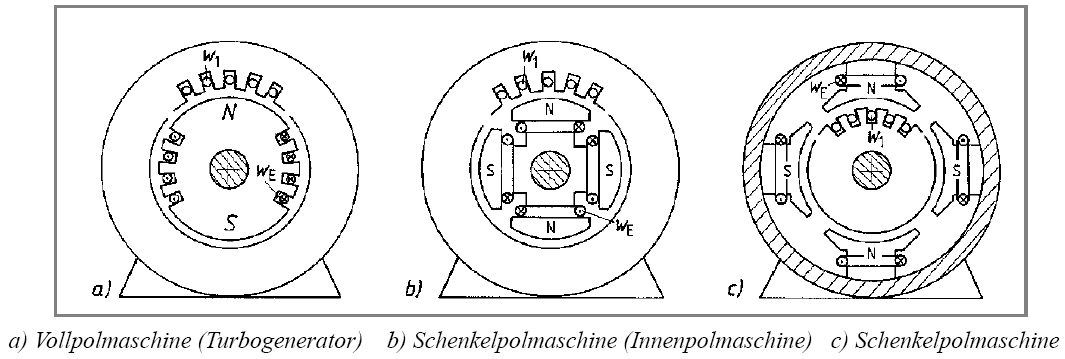
\includegraphics[width=12cm]{./Bilder/Aufbau_DSM.png}\\
		\begin{tabular}{ p{1cm} p{4cm} p{10cm}}
			- & Innenpolmaschine: & Der Läufer ist ein Dauermagnet, oder wird mit
			Gleichstrom und über Schleifer zu einem solchem gemacht. Dieser läuft mit dem aussen
			alsiegendem Drehfeld mit\\
			- & Aussenpolmaschine: & Der Läufer erzeugt ein Drehfeld, welches sich immer
			am konstanten Statorfeld ausrichtet. Worauf sich des Läufer dreht\\
			- & Turbomaschine: & Die Schleiferlose Variante. Mit Hilfe eines
			Hilfsgenerator auf der gleichen Welle wird ein Drehstrom erzeugt, welcher
			auf dem Läufer selbst gleichgerichtet wird. Damit wird dan ein konstantes
			Magnetfeld (Dauermagnet) erzeugt (wie die Innenpolmaschine)\\
		\end{tabular}
	\subsection{Ersatzschaltbild}
		\begin{minipage}{11cm}
			\abb{Bilder/Ersatz_DSM.png}{8cm}{Ersatzschaltung DSM}    
			Es gibt 2 Unterteilungen:\\
			\begin{tabular}{p{1cm} p{9cm}}
			    -& Wirkleistung: Gibt die DSM leistung ab oder nimmt sie auf. Zu erkennen
			    ist das am Phasenwinkel zwischen $U_{KL}$ und $U_P$. Ist $U_P$ voreilend, so ist
				es ein \textbf{Generator}, anderseits ein \textbf{Motor}.\\
				-& Blindleistung: Blindleistung Auf- oder Abgabe. Bei
				\textbf{Übererregung} oder auch \textbf{kapazitiven Betrieb} gibt der
				DSM Blindleistung ab. Bei \textbf{Untererregung} oder auch \textbf{induktiven Betrieb} nimmt er auf.\\
			\end{tabular}
	    \end{minipage}
		\begin{minipage}{8cm}
	    	\abb{Bilder/Zeigerdiagram.png}{6cm}{Betriebszustände einer DSM}
	    \end{minipage}\\
	
	\subsection{Betriebsverhalten}
 		\begin{tabular}{l l l l}
 	        Leerlauf&	
 	        \begin{minipage}{5cm}
 	        	\abb{Bilder/Leerlaufkennlinie.png}{4cm}{Im Betriebspunkt
 	        	liniarisierte Leerlaufgerade}
 	        \end{minipage} &
 			$I_E = \frac{U_P \cdot \sqrt{3} \cdot I_{E0N}}{U_N}$ &
 			\begin{minipage}{9cm}
 	       		Die Formel ist für die liniarisierte Gerade\\
 	           	$I_E: $Erregerstrom\\
 	           	$U_P: $verkettete Nennspannung des DS- Netzes\\
 	           	$I_{E0N}:$Leerlauferregerstrom für Nennspannung
 	        \end{minipage}\\
		\end{tabular}\\
\\
		\begin{tabular}{l l l l}
 			Kurzschluss &
 			\begin{minipage}{5cm}
             	\abb{Bilder/Kurzschlussgerade.png}{4cm}{Kurzschlussgerade}
            \end{minipage}&
 			$X_d=\frac{U_P}{I_{K0}}$ &
 			\begin{minipage}{9cm}
             	Gilt unter Vernachlässigung des Wicklungswiderstand\\
             	Die Kurzschlussgerade ist liniar
            \end{minipage}\\
 		\end{tabular}
		
		
			
		\subsubsection{Inselbetrieb}
			\begin{minipage}{10cm}
            
            	\abb{Bilder/Belastungskennlinie_DSM.png}{9cm}{Belastungskennlinie bei konst. Erregerstrom}
            \end{minipage}
			\begin{minipage}{6cm}
            	\abb{Bilder/Regulierungslinie_DSM.png}{6cm}{Regulierungskennlinie
            	für konst. $U_{Kl}$}
            \end{minipage}\\
			Die Klemmenspannung nimmt bei kapazitiven Lasten zu, bei induktiven stark
			ab. Für eine konstante $U_{Kl}$ muss der Erregerstrom wie die
			Regulierungskennlinie angepasst werden.
		\subsubsection{Netzbetrieb}
			Im Netzbetrieb wird die Frequenz, Klemmenspannung, Umlaufsinn und Phasenlage
			vom Netz vorgegeben. Das heisst bevor man mit einer DSM ans Netz will, muss man sie so
			synchronisieren, dass alle jene Parameter mit dem Netz überreinstimmen.
			Sind die Maschine und Netz synchronisiert und zusammengeschaltet, kann mit
			Hilfe von $I_E$ und der mechanischen Leistung der Blindstromanteil
			eingestellt werden:\\
			\begin{minipage}{8.2cm}
            	\abb{Bilder/Ortskurve_DSM.png}{8cm}{Ortskurve einer DSM im starren
            	Netz}
            \end{minipage}
			\begin{minipage}{9.7cm}
            \begin{tabular}[c]{p{0.2cm} p{9.5cm}}
				-& Da $U_{Kl} = U_1$ konstant ist, ist der Ursprung des Zeigers $\frac{j
				\cdot U_p}{X_d}$ immer am gleichen Ort.\\ 
				-& Mit dem Erregerstrom kann man die Länge des Zeigers $\frac{j \cdot
				U_p}{X_d}$ einstellen.\\
				-& Die mechanische Leistung ist proportional zum Abstand der
				Zeigerspitze zur Imaginärachse. \\
				-& Die Blindleistung ist proportional zum Abstand  der
				Zeigerspitze zur Reelenachse.\\
				-& Ist nun die mechanische Leistung konstant und man ändert den
				Erregerstrom, so wandert die Zeiger auf einer Linie parallel zur Imag-Achse hin und her.\\
				-& Überschreitet der Zeiger die Stabilitätslinie, schlipft der Läufer durch
				und es gibt grosse Lärm- und Wärmeentwicklung, da die mechanische Leistung zu
				gross wird für den Erregerstrom.\\
				-& Bleibt der Erregerstrom konstant und die mechanische Leistung ändert
				sich, so wandert der Zeiger auf dem Kreis um (0,$\frac{U_Kl}{j \cdot X_d}$).
				Jedoch wiederum nur bis zur Stabilitätsgrenze, da dort die Wirkleistung für
				diesen Erregerstrom maximal ist.         
             \end{tabular}	
			 \end{minipage}\\
\\
			\\
			$U_P = \sqrt{\frac{U^2_{Netz}}{3} + X_d^2 \cdot I^2 + 2 \cdot
			\frac{U_{Netz}}{\sqrt{3}}\cdot X_d \cdot I \cdot \sin(\varphi)}$
	
%%%%%%%%%%%%%%%%%%%%%%%%%%%%%%%%%%%%%%%%%%%%%%%%%%%%%%%
%Asynchronmotor
%%%%%%%%%%%%%%%%%%%%%%%%%%%%%%%%%%%%%%%%%%%%%%%%%%%%%%%
\newpage

\section{Drehstrom- Asynchronmaschinen (DAM)}
	\subsection{Aufbau der DAM}
		\begin{tabular}[c]{| p{3cm} | p{5cm} | p{4cm} | p{5cm} |}
        \hline
        Name & Aufbau & Positiv & Negativ\\
        \hline
        Schleifringläufer	& Ständerwicklung und Läuferwicklung sind für
        Drehfelder gewickelt. Die Läuferwicklunganschlüsse sind rausgezogen, um
        einem Widerstand einzuschliessen.
        & Mit deiesem Widerstand lässt sich die Drehzahl regulieren
        & Die Schleifkontakte reduzieren den Wirkungsrad und erhöhen den
        Verschleiss.\\
        \hline
        Kurzschlussläufer / Käfigläufer &
        Die Läuferwicklungen sind immer kurzgeschlossen.
        & Es kann ein beinahge reibungsloser und verschleisfreier Betrieb
        ermöglicht werden
        & Die Drehzahl ist beinahe die Drehfeldfrequenz durch die Polzahl\\
        \hline
        \end{tabular}
 	\subsection{Funktionsprizip} 
 		Das vom Ständer erzeugter Drehfeld erzeugt im
 		stillstehenden, kurzgeschlossenen Läufer einen Drehstrom. Der Schlupf
 		ist bei einem stillstehendem Läufer 1. Dieser Drehstrom erzeugt im Läufer ein
 		Drehmoment. Dieses Drehmoment beschleunigt den Läufer.Durch verringert sich
 		Schlupf, was wiederum ein kleineres Drehmoment nachsichtzieht.
 		Bei einem Läufergeschwindigkeit, welche gelcih schnell ist wie das
 		Drehfeld, reslutiert eine relative Geschwindigkeit von 0
 		(Schlupf von 0)$\rightarrow $ kein Drehmoment. Das heisst der DAM bewegt
 		sich immer mit möglichst kleinem Schlupf.
	\subsection{Ersatzschaltbild}
		Da der DAM nach dem Induktionsgesetz funktionniert, kann man ihn gut als
		Trafo- Ersatzschaltbild darstellen. Der veränderliche Wirkwiderstand
		(Lastwiderstand) ist die mechanische Last. Das heisst die Verlustleistung
	 über dem Widerstand ist die Mechanische Nutzleistung (minus die
	 Reibungsverluste). Diese ist, wie man sieht von dem Schlupf abhnängig.
		\abb{Bilder/ersatzschaltbild_DAM}{12cm}{Ersatzschaltbild des DAM mit Last}
		
	für Dreieckschaltung:\\
	\begin{tabular}{p{3cm} p{13cm}}
    	Kippmoment: & $M_k= Faktor \cdot M_N$\\
    	Kloss`sche Gleichung: &$\frac{M}{M_k}=\frac{2 s s_k}{s^2+s_k^2} $\\
    \end{tabular}\\
	\begin{tabular}{p{3cm} p{13cm}}
    	für Sternschaltung: & $M_{Stern}= \frac{M_\Delta}{3}$
    \end{tabular}
	       
	\subsection{Drehmomentkennlinie}
		\begin{minipage}{5cm}
        	\abb{Bilder/Drehmomentkenn_DAM.png}{5cm}{$M = f(s)$}   
        \end{minipage}
		\begin{minipage}{13cm}
        	$M_K = Kippmoment = Maximales Drehmoment$\\
        	$M_K \approx \frac{3 \cdot U_1^2}{4\cdot \pi \cdot n_1 \cdot
        	X_\sigma}$\\
        	$X_\sigma = X_{\sigma 1} + X_{\sigma 1}^`$\\
        	$\frac{M}{M_K}\approx \frac{2}{\frac{s}{s_k}+\frac{s_k}{s}}$\\
        	$s_k = \frac{R_2^`}{\sqrt{R_1^2 + X_1^2}} \approx
        	\frac{R_2^`}{X_\sigma}$
        	
        \end{minipage}
    	
\newpage
	\subsection{Ortskurve des DAM, Heyland- Kreis}
	\begin{minipage}{9cm}
    	\abb{Bilder/Heylandkreis.png}{8cm}{Heylandkreis mit Leistungs- und
    	Momenteneinteilung}
    \end{minipage}
	\begin{minipage}{8cm}
		\abb{Bilder/Heylandkreis_schlupf.png}{7cm}{Heylandkreis mit
		Schlupfskalierung}
    \end{minipage}\\
	\begin{minipage}{10.5cm}
	\begin{enumerate}	  

          \item Den Massstab für den Strom wählen zB. $m_I=\frac{0.2 A}{mm}$

          \item Den Massstab für die Leistung berechnen: $P_{gesamt}=3U_N
          I_{Ph}$ $m_P=3U_N m_I$
          \item Den Massstab für das Drehmoment berechnen:
          $M=\frac{P_\delta}{2\pi n_0};$  $m_M= \frac{p\cdot m_P}{2\pi f}$  p =
          Polpaar

          \item $s=0 \rightarrow s_{0}$ messen und einzeichnen
          \item $s=1 \rightarrow s_{1}$ messen und einzeichnen
          \item Verlustleistung bei $s_{0}$ herauslesen ($P_{Fe}$) (ev. wenn
          nicht schon getan, mit \\ $P_{FE} = U \cdot I_{Wirk}$ den
          Leistungs-Massstab bestimmen.)\\
          \item $\perp$ vom Mittelpunkt von $\overline{s_{0}s_{1}}$
          \item Schnittpunkt auf $s_{0}- Achse (Richtung -j) = M$
          \item Kreis um M mit Schnittpunkt $s_{0}$ und $s_{1}$
          \item $I_N =$ Tangente auf dem Kreis vom Ursprung (0,0)
          \item $P_{v1}$ bei $s_{1}$ ausrechnen = $P_{R_1}$ von der Parallele zur J-Achse, welche durch M geht nach oben
          abtragen.
          \item Verbindung des Punktes zu $s_{0}$ verlängern $\rightarrow$
          		$s_{\infty}$
          \item \textit{ Bei Vereinfachung $R_{Cu}=0:\\ s_{0}$ auf Imaginär- Achse;
          		$s_{\infty}$ auf Imaginär-Achse}
          \item Schlupf- Skalierung: $\perp$ auf $\overline{s_{\infty}M}$
          \item Schnittpunkt mit Verlängerung $\overline{s_{1}s_{\infty}}= 1$
          \item Schnittpunkt mit $\overline{s_{0}s_{\infty}}= 0$
          \item Dazwischen lineare Unterteilung
    \end{enumerate}
    \end{minipage}
	\begin{minipage}{7cm}
    	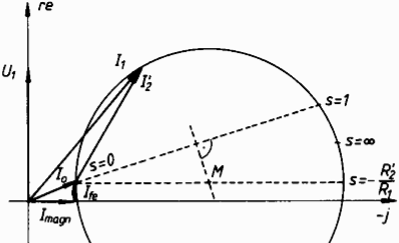
\includegraphics[width=6cm]{../ElMasch/bilder/StromortskurveDAM.png}\\
    	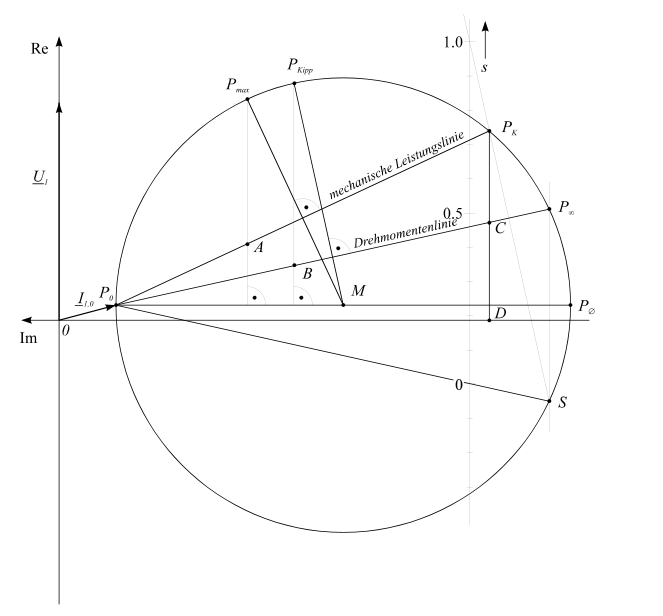
\includegraphics[width=8cm]{../ElMasch/bilder/OssannakreisPkipp.png}
    \end{minipage}

        
		
% 		
% 		
% \section{Persönliche Zusammenfassung}
% 4 A4-Blätter als Zusammenfassung/Formelsammlung.

\end{document}
